\subsection{Logica}

Het Wiselib systeem is onderverdeeld in verschillende klassen. Anonieme gebruikers zijn voorgesteld door de klasse \textbf{User}. 
Er is nood om de anonieme gebruiker voor te stellen omdat die toegang heeft tot basisfunctionaliteiten zoals het opzoeken van publicaties.
Eenmaal een gebruiker ingelogd is wordt hij door de klasse \textbf{RegisteredUser} voorgesteld. 
De applicatie maakt een onderscheid tussen een gebruiker en een persoon (\textbf{Person}).
Het is namelijk mogelijk dat een auteur in de gegevensbank opgeslagen is, maar niet als gebruiker ingeschreven is. 
Dit kan bijvoorbeeld gebeuren wanneer een gebruiker een publicatie met co-auteurs uploadt.

Publicaties zijn voorgesteld door de klasse \textbf{Publication}. Er wordt een onderscheid gemaakt tussen twee typen publicaties : \textbf{JournalPublication} en \textbf{ProceedingPublication}.
Dit onderscheid is noodzakelijk omdat deze publicaties verschillende karakteristieken hebben. \textbf{ProceedingPublication}s hebben bijvoorbeeld publishers en editors, wat niet het geval is bij \textbf{JournalPublication}s.

Omdat de rank van een journal of een conference een invloed heeft op de rank van een publicatie worden zij ook door hun eigen klasse gerepresenteerd (respectievelijk \textbf{Journal} en \textbf{Conference}).

%\href{class-diagram.png}{
\begin{figure}[p]
    \centering
    %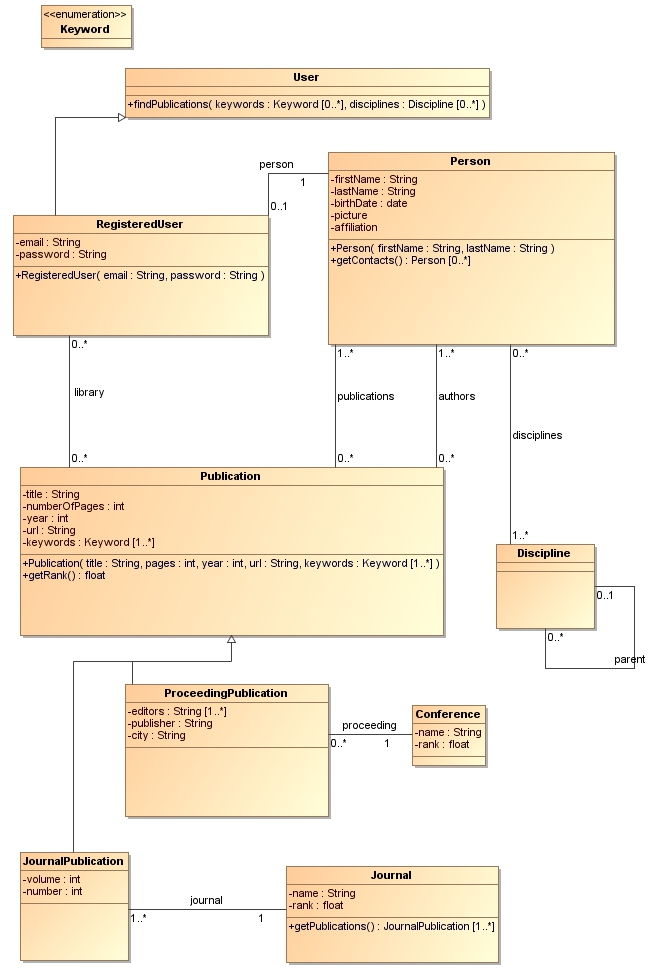
\includegraphics[width=155mm]{class-diagram}
    \href{run:./class-diagram.png}{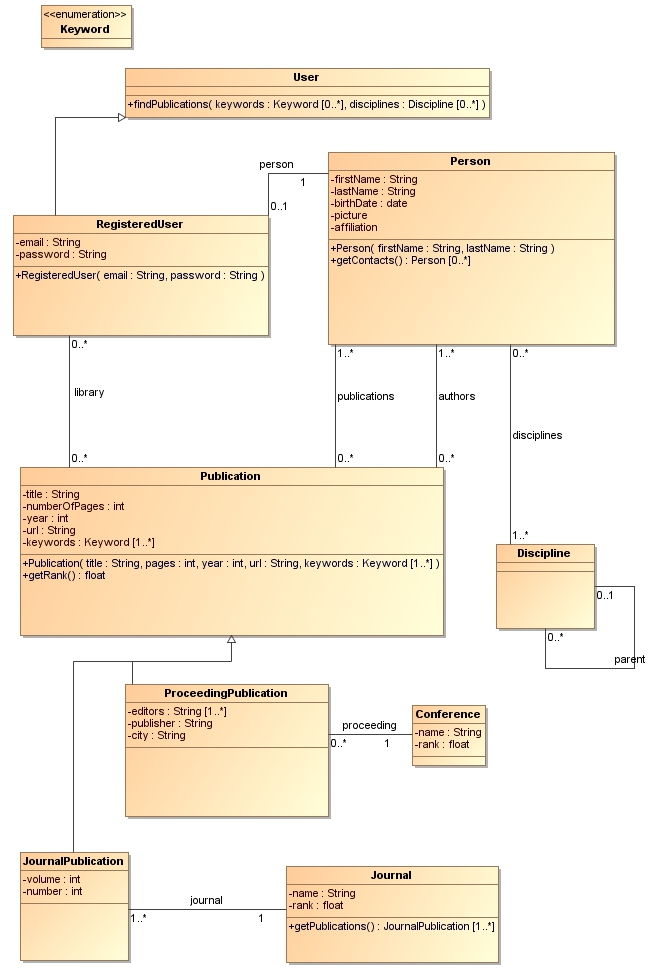
\includegraphics[width=\columnwidth]{class-diagram.png}}
    \caption{Klasse Diagram}
    \label{fig:class-diagram}
\end{figure}
